\chapter{Detumbling}

The orbital injection of the cubesat is done with the help of a dispenser  from the final stage of the rocket. The dispensing manoeuvre is net 100\% inear and hence imparts angular momentum to the cubesat. For effective data transfer and data collection, the cubesat needs to be free of any angular momentum. Detumbling is the process of engaging attitude controllers on the cubesat to reduce its tumbling. The attitude control (actuation) system that we have is a magnetorquer board. The magnetorquer is a set of three solenoids that produces a sufficient magnetic field in mutually perpendicular directions, which interacts with the magnetic field of the earth to generate sufficient torque for the cubesat to detumble.

\vspace{15pt}

Effective detumbling can be done by energising the torquer rods in such a fashion as to maximise the torque generated at each instant. This is achieved through a control algorithm called “B.dot control”. This algorithm computes the current that is required in each coil from the earth’s magnetic field around the cubesat (measured from magnetometer) as well as the angular velocity components (measured by gyro of the cubesat.)

\vspace{25pt}

\begin{figure}[h!]
	\centering
	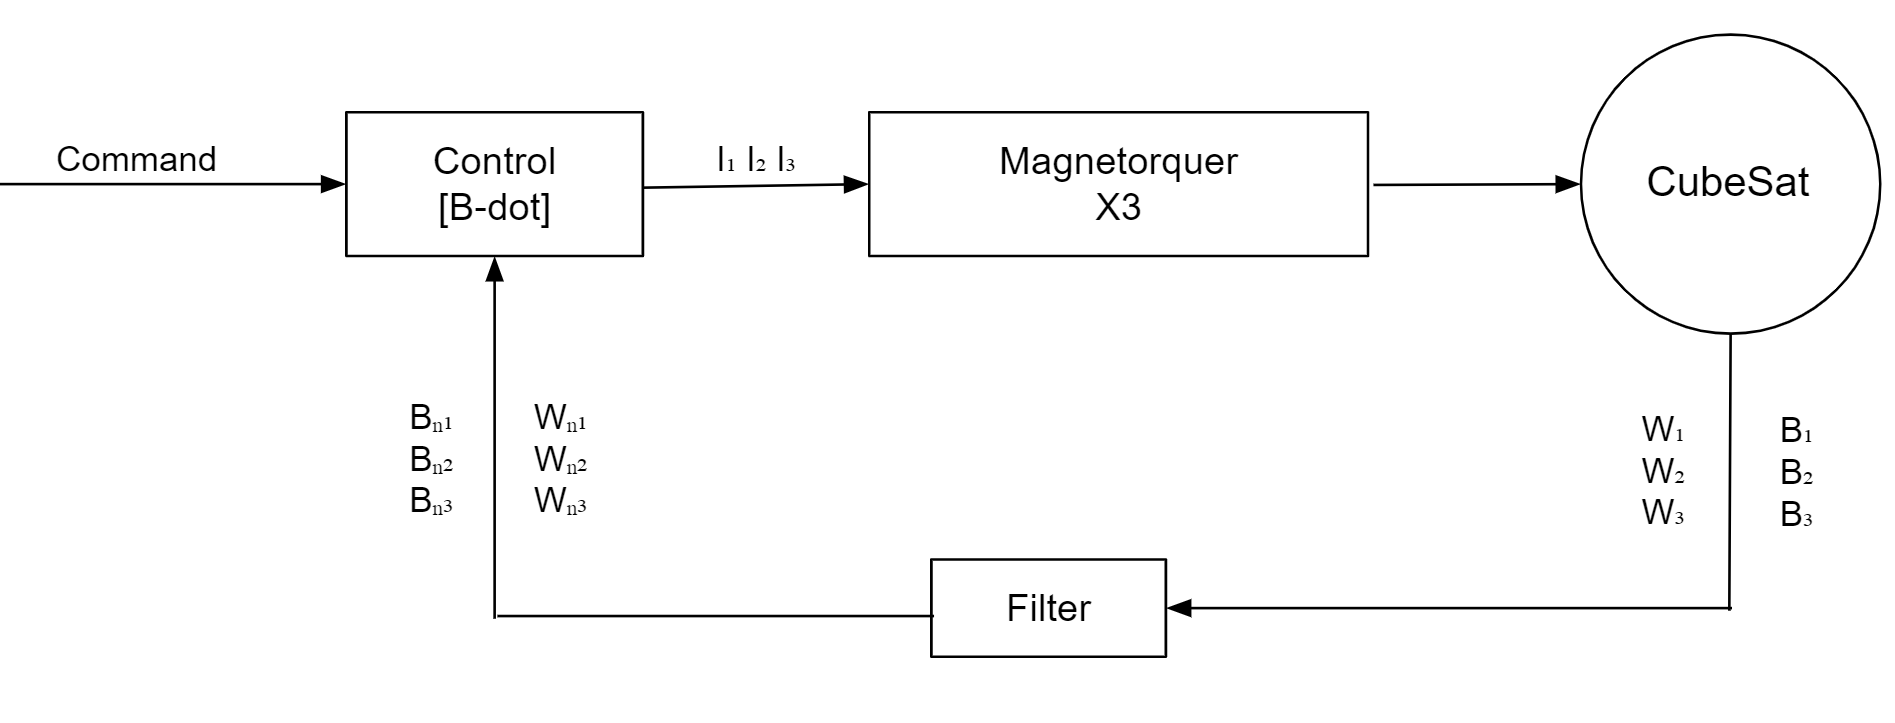
\includegraphics[width=4in,height=1.8in]{./images/flowChart}
	\caption{Detumbling system}
	\label{fig-flow-chart}
\end{figure}
 
 \vspace{25pt}
 
Here $[\omega_1, \omega_2, \omega_3]$ = Angular velocity about body axis of the cubesat

\hspace{25pt}$[B_1,B_2,B_3]$ = Magnetic field vector about body axis of the cubesat

\hspace{25pt}$[I_1,I_2,I_3]$ = Current in each magnetorquer coil

\vspace{15pt}

The sensor data ([$\omega$] and [B]) obtained from the Gyro and Magnetometer will contain biases and hence is necessary to calibrate them. The filtering algorithm yields corrected values of the sensor data. The algorithm shall depend upon the sensors used in each one. 

\vspace{15pt}

The b-dot algorithm relates the angular velocity and magnetic field to the magnetic moment ($\mu$) as being orthogonal to each other.

ie,$$\frac{\vec{\mu}}{|\mu|} = \frac{\vec{\omega}\times\vec{B}}{|\vec{\omega}\times\vec{B}|}$$

\vspace{1cm}
\hspace{45pt}Using a control parameter k
\vspace{1cm}

$$\vec{\mu} = k\cdot [\ \frac{\vec{\omega}\times\vec{B}}{|\vec{\omega}\times\vec{B}|} ]\ $$

$$\vec{\mu}= [mu_1 \mu_2 \mu_3] = [N_1I_1A_1  N_2I_2A_2  N_3I_3A_3]$$

where $N_1,N_2,N_3$ are number of turns on each coil

\hspace{32pt}$A_1,A_2,A_3$ are area of cross section of each coil

\vspace{15pt}
Hence we will obtain [$I_1 I_2 I_3$].Three PWM pinouts from the magnetorquer control IC generate sufficient voltage to energise the corresponding coils with $I_1 ,I_2, I_3$
